%-----------------------circuit 2--------------------------
\section{Single Phase Half Wave Controlled Rectifier with RL load}

\subsection{Circuit used for simulation}

% figure that is centered on the page
\begin{figure}[h]
    \centering
    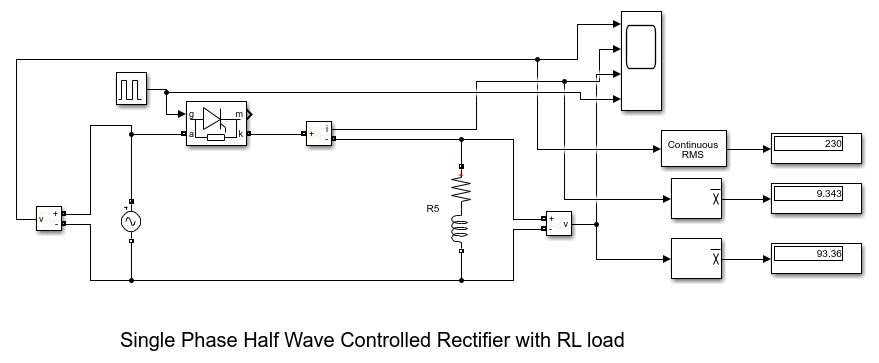
\includegraphics[width=0.7\textwidth]{images/experiment-1/circuit-diagram-simulation-06.png}
    \caption{Circuit used for simulation (Firing Angle = 30$ ^\circ $))}
    \label{Fig_simulation_circuit_single-phase-half-wave-controlled-rectifier-with-RL-load}
\end{figure}

\subsection{Components Required}

\begin{table}[h]
    \renewcommand{\arraystretch}{1.3}
    \label{table_components_required_circuit_6}
    \centering
    \begin{tabular}{|c|c|c|c|}
        \hline
        Sr. No & Parameters                     & Ratings            & Quantity \\
        \hline
        \hline
        1      & AC Single Phase Voltage Source & 230V ($ V_{rms} $) & 1        \\
        \hline
        2      & Resistor                       & 10$ \Omega $       & 1        \\
        \hline
        3      & Inductor                       & 10mH               & 1        \\
        \hline
        4      & Diode                          & -                  & 1        \\
        \hline
        5      & Voltmeter                      & -                  & 2        \\
        \hline
        6      & Ammeter                        & -                  & 1        \\
        \hline
        7      & Thyristor                      & -                  & 1        \\
        \hline
    \end{tabular}
    \caption{Components for Single Phase Half Wave Controlled Rectifier with RL load}

\end{table}




\subsection{Observations}

\begin{table}[h]
    \renewcommand{\arraystretch}{1.3}
    \label{table_observation_6}
    \centering
    \begin{tabular}{|c|c|c|}
        \hline
        Parameters                              & Theoretical Values & Simulation Values \\
        \hline
        \hline
        AC Input Voltage ($ V_{in,rms} $)       & 230V               & 230V              \\
        \hline
        Output Average Voltage ($ V_{o,avg} $)  & 96.6V              & 93.36V            \\
        \hline
        Output Average Current ($ I_{o,avg}  $) & 9.66A              & 9.343A            \\
        \hline
        AC Input Power ($ P_{AC}  $)            & 2214.44 (W)        & 2296 (W)          \\
        \hline
        DC Input Power ($ P_{DC}  $)            & 926.98 (W)         & 872.3 (W)         \\
        \hline
        Efficiency (\%)                         & 41.86              & 37.99             \\
        \hline
    \end{tabular}
    \caption{Observations for Single Phase Half Wave Controlled Rectifier with RL load}

\end{table}


Upon providing the firing gate pulse to the thyristor, it is observed that the circuit begins conducting. Due to the presence of an inductive component in the load, the output current lags behind the output voltage, leading to the conduction of the diode until the output current approaches zero. Consequently, the output voltage becomes negative during this duration. After the output current falls to zero, the thyristor ceases conduction, and the output voltage returns to zero as well.
The efficiency of controlled
rectifier with RL load is 37.99\%.


% \pagebreak

\subsection{Resultant Waveforms}

% figure that is centered on the page
\begin{figure}[h]
    \centering
    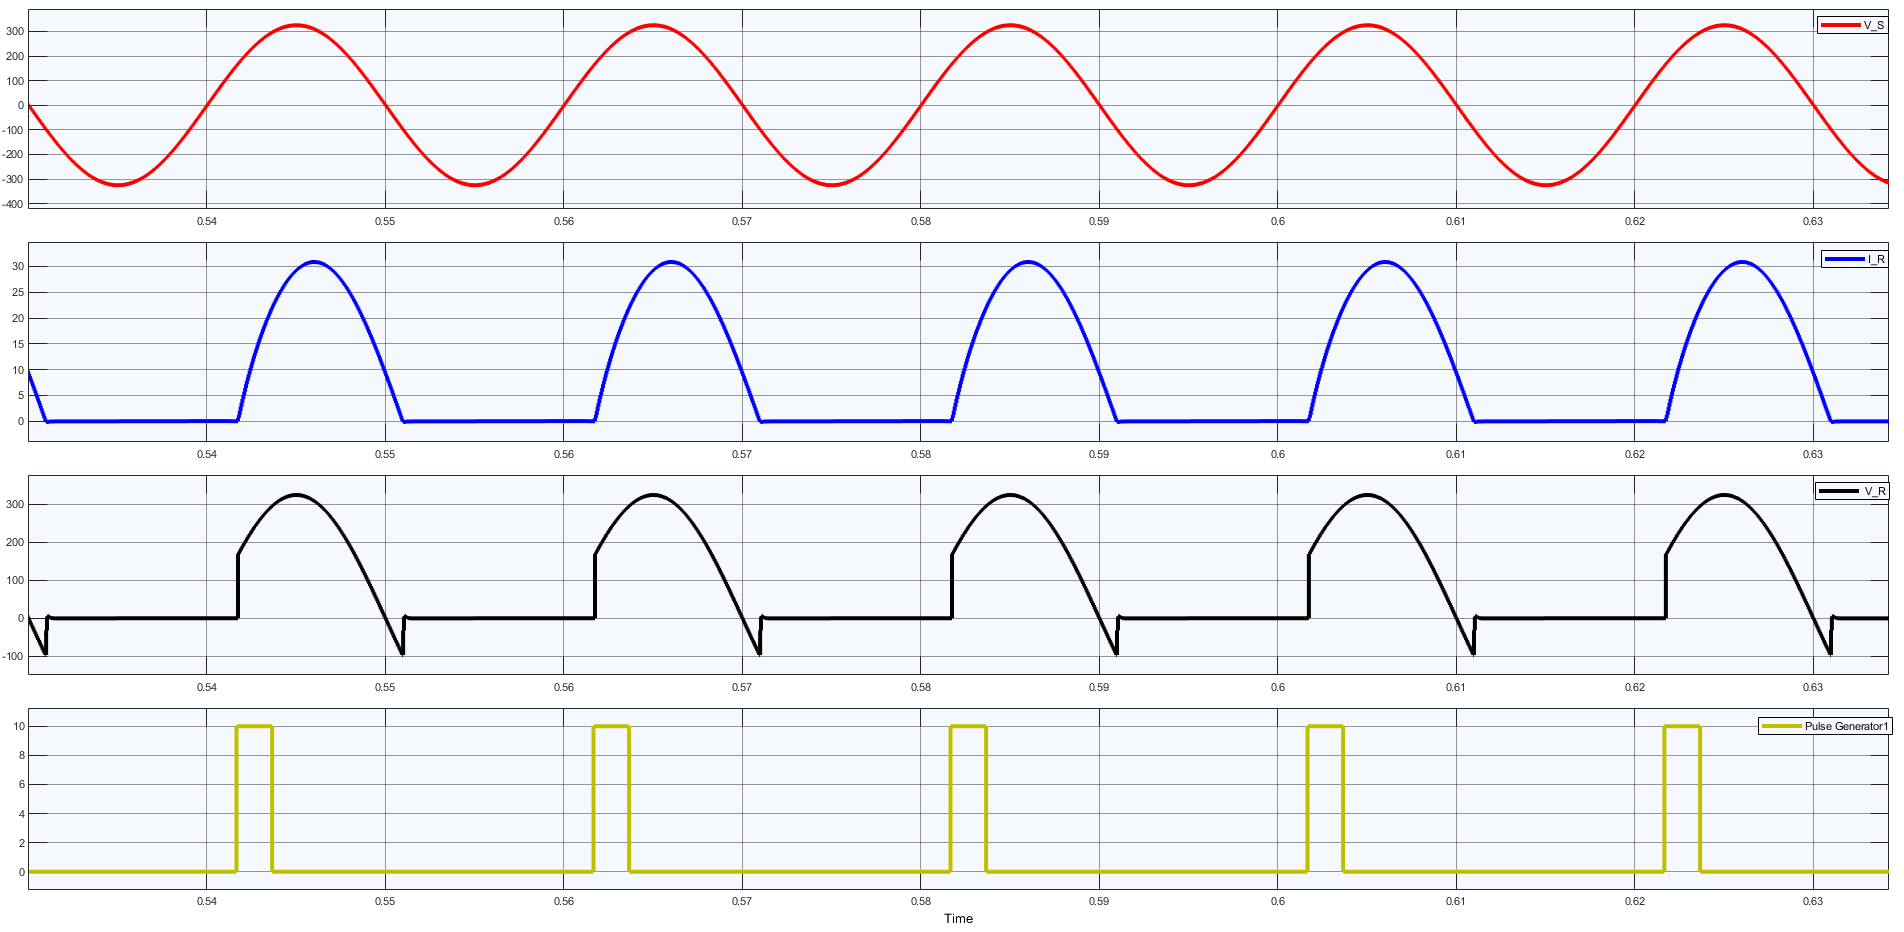
\includegraphics[width=1\textwidth]{images/experiment-1/circuit-scope-simulation-06.png}
    \caption{Scope Waveforms for Single Phase Half Wave Controlled Rectifier with RL load}
    \label{Fig_waveform_single-phase-half-wave-controlled-rectifier-with-RL-load}
\end{figure}

\pagebreak
